\documentclass[../main.tex]{subfiles}
\hbadness=1000000
\vbadness=1000000

\begin{document}

\section{Methodology}
\subsection{Network of coupled Kuramoto oscillators: synchronization}
We have studied the synchronization properties and information transmission in the circuits of the V- and the C-motifs.
Initially, we conducted a preliminary study of the synchronization states or solutions in these motifs using the Kuramoto model \citep{kuramoto1975international} to describe the dynamics of each of the three elements that comprise them.
Subsequently, a similar study was performed, now considering each element as a balanced network of neurons whose dynamics are described by the Hodgkin-Huxley \citep{hodgkin_quantitative_1952} model.
For the latter network circuits, we investigated the information transmission under different delay and frequency mismatches.
Table \ref{tab:circuits} summarizes all the conditions for which we have investigated these circuits.
This table uses the nomenclature relative to the equations given by the Kuramoto model.
\begin{table}[h]
\caption{Different conditions of interest for the V-motif and C-motif circuits}
\begin{tabular}{|c|c|c|c|}
\hline
\multirow{2}{3cm}{\centering Circuit}  & \multirow{2}{2.5cm}{\centering Coupling}  & \multirow{2}{2.5cm}{\centering Detuning} & \multirow{2}{3cm}{\centering Delay} \\
& & & \\
\hline
    \multirow{2}{2cm}{\centering V-motif}
    &   
    \multirow{2}{2.5cm}{\centering$K=0.5K_0$}
    &
    \multirow{3}{3cm}{\centering
    $\begin{aligned}
    \Omega_0 &= \Omega_2 = \Omega_3 \\
    \Omega_1 &= \Omega_0 + \Delta\Omega_1
    \end{aligned}$}
    &
    \multirow{6}{3cm}{\centering
    $\begin{aligned}
        \delta &= \delta_{12} = \delta_{21} \\
        \quad  &= \delta_{23} = \delta_{32} 
    \end{aligned}$ }
    \\ 
    & & & 
    \\
    \cline{2-2}
    \multirow{4}{3cm}{\centering
    $\begin{aligned}
        K &= K_{12}=K_{32}\\
        K_0 &=K_{21}=K_{23}
    \end{aligned}$
    }
    &  
    \multirow{2}{2.5cm}{\centering $K= K_0$}
    & & 
    \\
    & &  
    \multirow{3}{3cm}{\centering
    $\begin{aligned}
    \Omega_0 &= \Omega_1 = \Omega_3 \\
    \Omega_2 &= \Omega_0 + \Delta\Omega_2
    \end{aligned}$
    }
    & 
    \\
    \cline{2-2}
    & \multirow{2}{2.5cm}{\centering $K=1.5 K_0$} & & 
    \\    
    & & &  
    \\
\hline    
%%%%%%%%%%%%%%%%%%%%%%%%%%%%%%%%%%%%%%%%%%%%%%%%%%%%%%%%%%%%%
    \multirow{3}{3cm}{\centering C-motif}
    &   
    \multirow{2}{2.5cm}{\centering $K'= 0.05K_0$}
    &
    \multirow{4}{3cm}{\centering
    $\begin{aligned}
    \Omega_0 &= \Omega_2 = \Omega_3 \\
    \Omega_1 &= \Omega_0 + \Delta\Omega_1
    \end{aligned}$}
    &
    \multirow{8}{3cm}{\centering
    $\begin{aligned}
        \delta &= \delta_{12} = \delta_{21} \\
        \quad  &= \delta_{23} = \delta_{32} \\
        \quad  &=  \delta_{13} = \delta_{31}
    \end{aligned}$ } 
    \\ 
    & & & % 2
    \\ \cline{2-2}
    & \multirow{2}{2.5cm}{\centering $K'= 0.25K_0$} & & 
    \\
    \multirow{5}{3cm}{\centering
    $\begin{aligned}
        K' &= K_{13}=K_{31}\\
        K_0 &=K_{12}=K_{21}\\
        \quad &= K_{23}=k_{32}
    \end{aligned}$
    }
    & & & % 4
    \\  \cline{2-2}
    &  
    \multirow{2}{2.5cm}{\centering $K'= 0.50K_0$}
    &  
    \multirow{4}{3cm}{\centering
    $\begin{aligned}
    \Omega_0 &= \Omega_1 = \Omega_3 \\
    \Omega_2 &= \Omega_0 + \Delta\Omega_2
    \end{aligned}$
    }
    & 
    \\  
    & & &  % 6
    \\ \cline{2-2}
    & \multirow{2}{2.5cm}{\centering $K' = 0.75K_0$} & & 
    \\    
    & & & % 8
    \\ 
\hline
\end{tabular}
\label{tab:circuits}
\end{table}

% \subsection{Network of coupled Kuramoto oscillators: synchronization}
Considering the V- and C-motifs as coupled Kuramoto oscillators simplifies the determination of synchronized or phase-locked solutions and the evaluation of their stability, eliminating the necessity for simulating their dynamics. 
This establishes a foundation for comprehending the collective properties that may arise from these motifs when employing more intricate modelling, as detailed later in our description.
% The Kuramoto model is a simple model that, under certain conditions, allows us to obtain analytical expressions, facilitating the understanding of the system's dynamics by analyzing the stability of fixed points within the parameter space.
% This parameter space is defined by the parameters we leave free according to our interest, namely, the delays (or lag) of the connections, conductances, and oscillation frequency (or detuning, the relative frequency compared to the basal frequency).
% The dynamical system associated with the first motif can be reduced to a one-dimensional system, while the others can be reduced to two-dimensional systems.
% This is because the first motif is completely defined by the phase difference between node 1 and node 2 ($\theta_{12}=\theta_1-\theta_2$), whereas in the other motifs, it is needed phase difference between two pairs of nodes, such as 1 and 2, and 1 and 3 ($\theta_{13}=\theta_1-\theta_3$).
% Any of the three possible options would equally describe the system as these variables are linked to each other.
% Applying equation \eqref{eq:kuramoto-model-phase-shift}, the dynamics of the 2-motif, $\theta_{12}(t) = \theta_1(t)-\theta_2(t)$, is described by:
% \begin{equation}
%     \dot{\theta}_{12} = \Delta\omega_{12} + k_{21}\sin(-\delta_{12}-\delta_{21}) - k_{12}\sin(\theta_{12}-\delta_{12}), 
%     \label{eq:kuramoto-2-motif}
% \end{equation}
% while the v- and c-motif can be described by the following differential equation system:
% \begin{equation}
% \begin{aligned}
%     \dot{\theta}_{12} & = \Delta\omega_{12} + k_{21}\sin(-\delta_{12}-\delta_{21}) + k_{31}\sin(-\theta_{13} - \delta_{31})\\
%        & \quad - k_{12}\sin(\theta_{12}-\delta_{12}) - k_{32}\sin(\theta_{12}-\theta_{13}-\delta_{32}), \\
%     \dot{\theta}_{13} & = \Delta\omega_{13} + k_{21}\sin(-\delta_{12}-\delta_{21}) + k_{31}\sin(-\theta_{13} - \delta_{31}) \\
%     & \quad -k_{13}\sin(\theta_{13}-\delta_{13}) - k_{23}\sin(\theta_{13}-\theta_{12}-\delta_{23}),
%     \label{eq:kuramoto-v-and-c-motif}
% \end{aligned}
% \end{equation}
% where the only difference is the values of the couplings between the outer nodes $1$ and $3$ ($k_{13}=k_{31}=0$ in the v-motif).
To find these phase-locked solutions we need to solve the equation system given by $\dot{\theta}_{12}=0$ and $\dot{\theta}_{13}=0$, which correspond to compute the fixed point solutions.
% A fixed point $\theta_{12}^{*}$ of the one-dimensional system \eqref{eq:kuramoto-2-motif}, can be:
% \begin{enumerate}
%     \item \textbf{Stable}: $\displaystyle\frac{d\dot{\theta_{12}}}{d\theta_{12}}(\theta_{12}*)<0$.
%     \item \textbf{Unstable}: $\displaystyle\frac{d\dot{\theta_{12}}}{d\theta_{12}}(\theta_{12}*)>0$.
%     \item \textbf{Marginally stable}: $\displaystyle\frac{d\dot{\theta_{12}}}{d\theta_{12}}(\theta_{12}*) = 0$ Further analysis is required to determined its behaviour. This can be done by looking into the second derivative or by simulations of the dynamics. 
% \end{enumerate}
% For the case of the v- and c-motifs, a bidimensional system, the analysis become more complex.
% Now 
In handling a two-dimensional system, the fixed points are determined by the pairs$(\theta_{12}^{*},\theta_{13}^{*})$.
In this category of dynamical systems, six distinct types of fixed points exist, classified based on the eigenvalues of the Jacobian matrix.
For the motifs of interest, the Jacobian matrix is defined by:
\begin{equation}
    J(\theta_{12}^{*},\theta_{13}^{*}) = 
     \begin{pmatrix}
    \displaystyle\frac{\partial\dot{\theta}_{12}}{\partial\theta_{12}} (\theta_{12}^{*},\theta_{13}^{*}) & \displaystyle\frac{\partial\dot{\theta}_{12}}{\partial\theta_{13}}(\theta_{12}^{*},\theta_{13}^{*})\\ 
    \displaystyle\frac{\partial\dot{\theta}_{13}}{\partial\theta_{12}}(\theta_{12}^{*},\theta_{13}^{*}) & 
    \displaystyle\frac{\partial\dot{\theta}_{13}}{\partial\theta_{13}}(\theta_{12}^{*},\theta_{13}^{*})
    \end{pmatrix}.
    \label{eq:jacobian-matrix}
\end{equation}
Let $\lambda_1$ and $\lambda_2$ be the eigenvalues of \eqref{eq:jacobian-matrix}. 
The fixed points $(\theta^{*}_{12}, \theta^{*}_{13})$ can be of the form \citep{zill2012differential}:
\begin{enumerate}
    \item \textbf{Stable node} or \textbf{sink}: $\lambda_1 = Re(\lambda_1) <0$, $\lambda_2 = Re(\lambda_2) < 0$.
    \item \textbf{Unstable node} or \textbf{source}:  $\lambda_1 = Re(\lambda_1)>0$, $\lambda_2 = Re(\lambda_2) > 0$.
    \item \textbf{Saddle point}: $\lambda_1 = Re(\lambda_1)$, $\lambda_2 = Re(\lambda_2)$ and $\lambda_1 < 0 < \lambda_2$. 
    \item \textbf{Center}: $\lambda_1 = Im(\lambda_1)$, $\lambda_2 = Im(\lambda_2)$.
    \item \textbf{Stable focus} or \textbf{spiral sink}: $\lambda_1 = Re (\lambda_1) <0$, $\lambda_2 = Re(\lambda_2) < 0$, $Im(\lambda_1)\neq0$, $Im(\lambda_2)\neq0$.
    \item \textbf{Unstable node} or \textbf{source}: $\lambda_1 = Re(\lambda_1) >0$, $\lambda_2 = Re(\lambda_2) > 0$, $Im(\lambda_1)\neq0$, $Im(\lambda_2)\neq0$
\end{enumerate}
% On the other hand, the sign of the determinant of the Jacobian matrix determines the orientation of the trajectories near the fixed point. 
% If $det(J) > 0$, the trajectories preserve their orientation; if $det(J) < 0$, the trajectories reverse their orientation.
% Additionally, the sign of the trace of the Jacobian matrix informs about the stability of the fixed point.
% If $tr(J) < 0$, the fixed point is stable, and if $tr(J) > 0$, the fixed point is unstable. 
% When $tr(J) = 0$, further analysis is needed to determine the stability.
Among all the various fixed points, our focus lies on those that are asymptotically stable, namely the stable nodes and the stables foci ,representing stable phase-locked states.
The remaining ones will be considered unstable, although, center fixed points are neutrally stable.
A dynamical system will only achieve the center fixed points if its initial conditions coincide with them; otherwise, the system will oscillate around them.
Therefore, we categorize them as part of the "unstable" group.

\subsection{Motifs of coupled population models}
The motifs of interest consist of three interconnected and balanced networks or populations, each comprising 100 neurons.
The neural population model is similar to the one used in \citep{pariz_high_2018}, where the dynamic of each neuron is described by the Hodgkin-Huxley neuron model, equations \eqref{eq:hodkin_huxley_eqs}-\eqref{eq:gate_eqs}.
As stated before, each population consists of 100 neurons, being 80 excitatory neurons and 20 inhibitory neurons.

The synaptic current $I_{\text{syn},i}$ (of the $i$-th post-synaptic neuron) is modeled with the double exponential function:
\begin{equation}
    \begin{aligned}[c]
        I_{\text{syn},i} &= \displaystyle\sum_{j}g_{ij}S_{ij}(t)(v_i-E_{\text{syn},i}),\\
        S_{ij}(t) &= \displaystyle\frac{1}{A}\Bigg[ \exp\Bigg(\displaystyle\frac{-(t-t_j^{*}-\tau_{ij})}{\tau_r}\Bigg)-
        \exp\Bigg(\displaystyle\frac{-(t-t_j^{*}-\tau_{ij})}{\tau_d}\Bigg)\Bigg], \\
        A &= \Bigg(\displaystyle\frac{\tau_r}{\tau_d}\Bigg)^{\frac{\tau_r}{\tau_d-\tau_r}} - \Bigg(\displaystyle\frac{\tau_r}{\tau_d}\Bigg)^{\frac{\tau_d}{\tau_d-\tau_r}},
    \end{aligned}
    \label{eq:double_exponential}
\end{equation}
where $v_i$ is the membrane potential of the post-synaptic neuron and $E_{\text{syn},i}$ is the reversal synaptic potential of the post-synaptic neuron.
$S_{ij}$ accounts for the effectiveness of both excitatory (assumed to be mediated solely by fast AMPA receptors) and inhibitory (assumed to be mediated solely by fast GABA$_{\text{A}}$ receptors) chemical synapses \citep{pariz_transmission_2021}.
While the intra-population connections are both excitatory and inhibitory, the inter-population connections are assumed to be only excitatory.
Variable $t_j^{*}$ refers to the time at which the $j$-th pre-synaptic neuron emits a spike and $\tau_{ij}$ is the axonal delay between the pre- and post-synaptic neurons.
The intra-population delay is set to 0.5 ms while the inter-population delay $\tau$ is varied from 0.5 to 14 ms.
This limit is fixed since it approximately corresponds to the inverse of the oscillating period of the population, \textit{i.e.} a delay that corresponds to a phase of $2\pi$.
\begin{figure}[htbp]
    \centering
    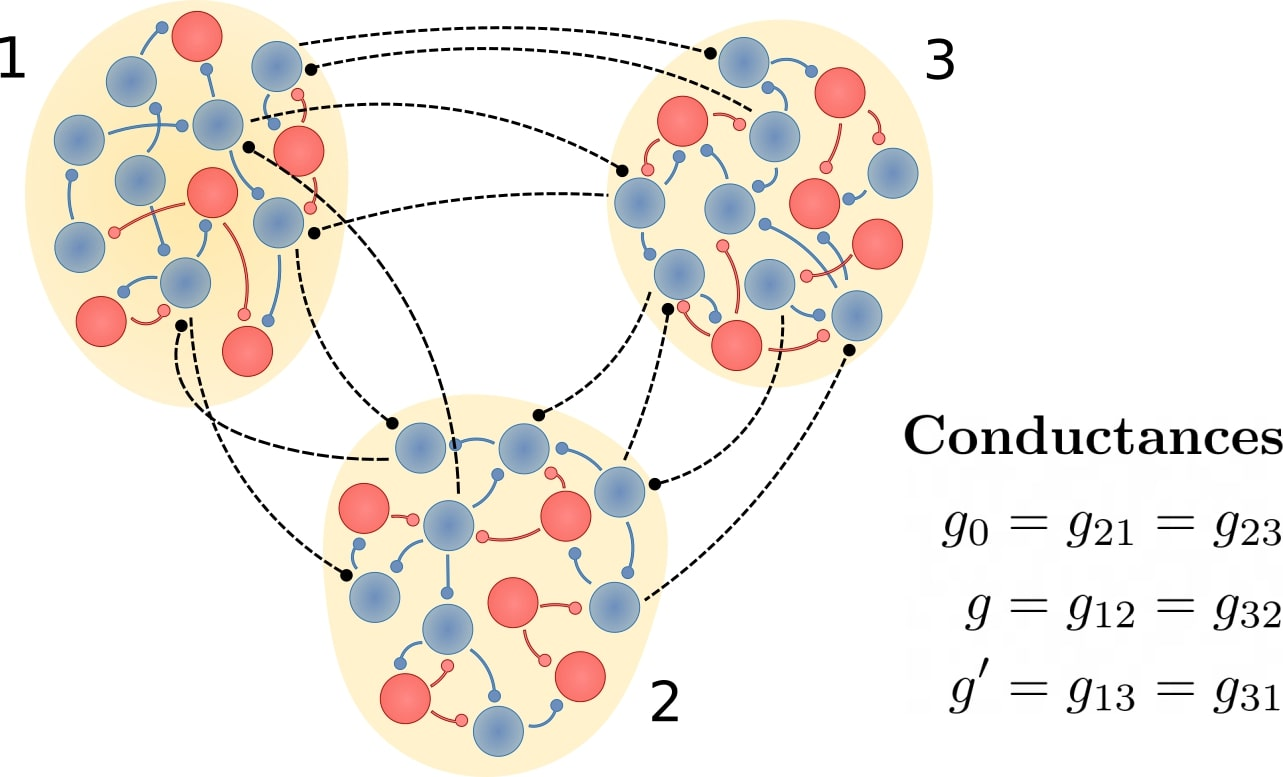
\includegraphics[width=90mm]{chapter2/figures/fig1}
    \caption{\textbf{Structure of the cortical circuit}.
    Cortical areas are represented by neural populations 1 and 3, while population 2 represents the thalamus.
    Excitatory neurons, inhibitory neurons, and their corresponding synaptic projections are depicted in blue and red respectively.
    The inter-population connections are exclusively excitatory, and their synaptic weights can be modified depending on the specific scenario.
    When there are no connections between populations 1 and 3, the circuit is referred to as a V-motif circuit.
    Alternatively, if these connections are present, it is classified as a C-motif circuit}
    \label{fig:vmotif}
\end{figure}

The parameters for the neurons and synaptic models are presented in Table \ref{table:parameters}; nonetheless, a degree of randomness is introduced to incorporate heterogeneity.
Each neuron is randomly connected to 10 $\%$ (5$\%$) of neurons in the same (different) population.
This connectivity pattern aligns with what is commonly assumed in the modelling of cortical neural networks \citep{izhikevich_simple_2003,lopez2017role}.
\begin{table}[htbp]
    \def\arraystretch{1.3}%  1 is the default, change whatever you need
    \centering
    \caption{Parameters of the model.}
    \begin{tabularx}{\textwidth}{|c|c|X|} \hline
         \textbf{Parameter} & \textbf{Value} & \textbf{Description} \\
         \hline
         $C$                & 1 $\mu$F/cm$^2$ & Capacitance\\      \hline
         $g_K$              & 36 $\mu$S/cm$^2$  & K conductance\\    \hline
         $g_{Na}$           & 120 $\mu$S/cm$^2$      & Na conductance\\   \hline
         $g_L$              & 0.3 $\mu$S/cm$^2$      & Leak conductance\\ \hline
         $E_K$              & -77 mV           & K reversal potential\\   \hline
         $E_{Na}$           & 50 mV            & Na reversal potential\\   \hline
         $E_L$              & -54.4 mV         & Leak reversal potential\\ \hline
         $E_{\text{syn},E}$ & 0 mV             & Excitatory reversal potential\\   \hline
         $E_{\text{syn},I}$ & -80 mV           & Inhibitory reversal potential\\ \hline
         $\tau_{inter}$     & 0-14 ms          & Inter population delay\\ \hline
         $\tau_{intra}$     & 0.5 ms           & Intra population delay \\ \hline
         $\tau_d$           & 3 ms             & Synaptic decay time \\ \hline
         $\tau_r$           & 0.5 ms           & Synaptic rise time\\ \hline
         $I_{\text{ext}}$   & 10-12 $\mu$A/cm$^2$    & Injected current\\ \hline
         $\mu$    			& 0 $\mu$A/cm$^2$     & Median of the gaussian white noise\\ \hline
         $\sigma$           & 0.5 $\mu$A/cm$^2$   & Standard Deviation of the gaussian white noise\\ \hline
         $g_{EE}$           & 3.75 $\mu$S/cm$^2$  & Synaptic weight: excitatory $\rightarrow$ excitatory\\ \hline
         $g_{EI}$           & 7.5 $\mu$S/cm$^2$   & Synaptic weight: excitatory $\rightarrow$ inhibitory\\ \hline
         $g_{IE}$           & 15 $\mu$S/cm$^2$    & Synaptic weight: inhibitory $\rightarrow$ excitatory\\ \hline
         $g_{II}$           & 15 $\mu$S/cm$^2$    & Synaptic weight: inhibitory $\rightarrow$ inhibitory\\ \hline
    \end{tabularx}
    \label{table:parameters}
\end{table}
Each neuron of the network receives an external constant injection current (or bias current) that varies between 10 to 12 $\mu$A/cm$^2$.
Additionally, each neuron receives a Gaussian white noise current of zero mean ($\mu$ = 0 $\mu$A/cm$^2$), and standard deviation $\sigma$ = 0.5 $\mu$A/cm$^2$.
In Figure \ref{fig:vmotif} we show a circuit schematics of the three populations and their connections.

Each of the three populations, either connected or disconnected, exhibits high levels of synchronization and a well-defined oscillatory behavior \citep{pariz_transmission_2021} (Figure \ref{fig:population-dynamics} A). 
The oscillation frequency exhibits a linear dependence on the constant current received by the neurons.
For the values we have considered, the oscillation frequency varies from 68 to 73 Hz (Figure \ref{fig:population-dynamics} B).
\begin{figure}[t]
    \centering
    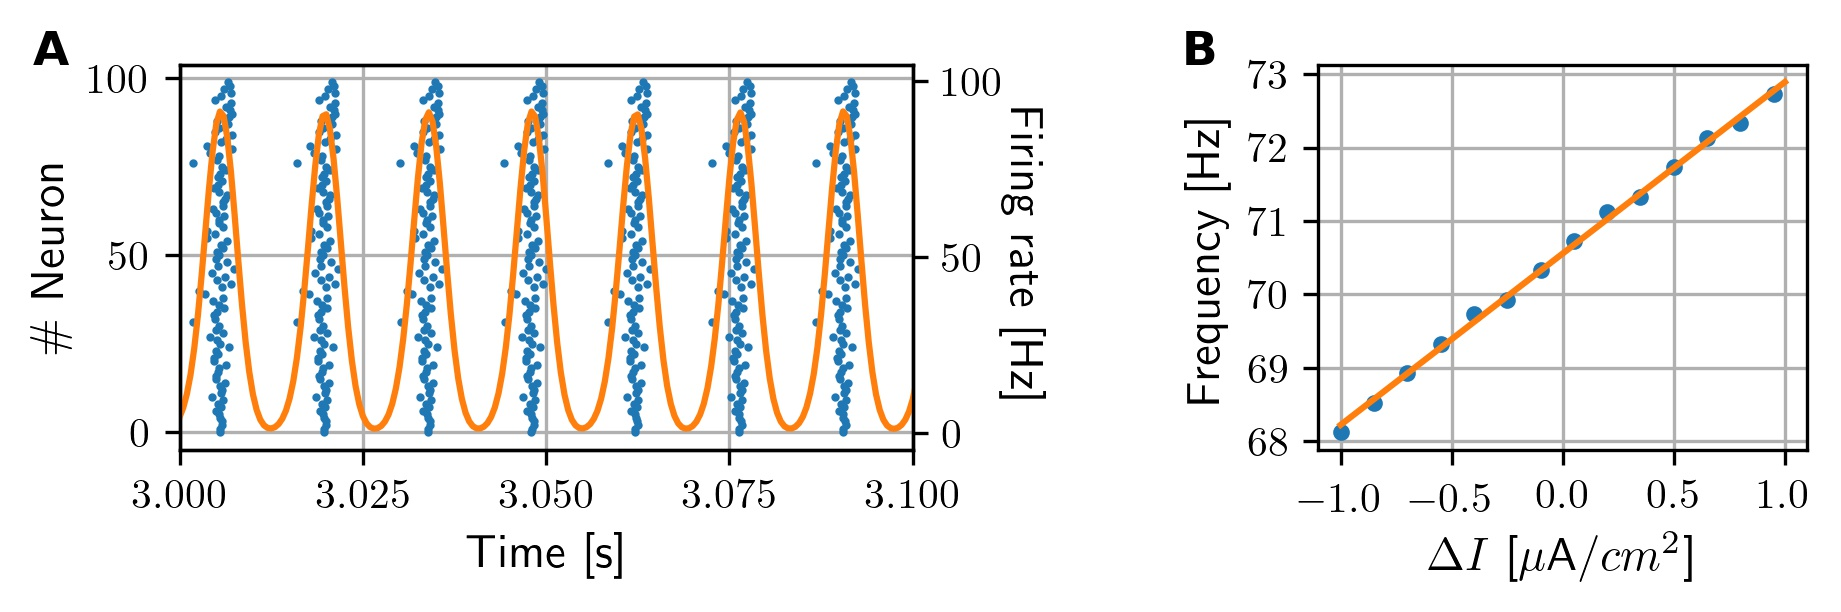
\includegraphics[width=\textwidth]{chapter2/figures/fig0s}
    \caption{\textbf{Properties of the population network}.
    Raster plot and firing rate of an isolated population with an injected bias current $I=I_0 = 11$  $\mu$A/$cm^2$ (A).
    Linear response of the collective oscillation frequency with respect to the detuning $\Delta I$ (B).}
    \label{fig:population-dynamics}
\end{figure}

Our parameter space is defined by the \textbf{detuning} or \textbf{frequency mismatch}
and the time \textbf{delays}.
We define the \textbf{detuning} or the \textbf{frequency mismatch} as the difference between the natural oscillation frequency of an isolated population to that of the other populations.

\subsection{Synchronization measurements}
Unlike motifs of coupled Kuramoto oscillators, in this case, we determine the synchronization or phase-locking by extensive numerical simulations.
To achieve this, we first need to extract the relative phase of each population.

\subsubsection{Firing rate}
This oscillatory dynamics of each network is captured by the firing rate $r(t)$.
To obtain it, we initially computed the multi-unit activity $s(t)$ of a population, \textit{i.e.} the total number of spikes that occur in the time interval between $t$ and $t+\Delta t$.
The firing rate of each population is the result of the convolution of the multi-unit activity $s(t)$ with a kernel function $w(t)$ \citep{dayan2003theoretical}:
\begin{equation}
r(t) = \displaystyle\frac{1}{N\Delta t}\displaystyle\int_{-\infty}^\infty s(t-t')w(t')dt',
\end{equation}
where $N$ is the total number of neurons in the network or population. 
This integral is usually called linear filter, and the window function $w(t)$ was considered here as a Gaussian function.
Depending on the value of $\sigma$ different frequencies can be filtered or removed.
We used $\sigma =$ 2.0 ms and $\sigma =$ 100.0 ms when injecting fast and slow signals into the system, respectively. 
In the absence of an external signal, $\sigma =$ 2.0 ms was also considered to compute the firing rate, since it preserves the natural oscillatory frequency of each population.
With $\sigma = 100.0$ ms we filter higher frequencies, enabling the capture of slower frequencies relative to the slow modulation injected into the network.

\subsubsection{Phase difference}
Extracting the corresponding phase involves identifying relative maxima in the time series and performing a linear extrapolation to associate a phase with each moment in time.
The phase of each neural population was computed from its collective oscillatory firing rate $r(t)$ by the interpolation
\begin{equation}
	\theta(t) = 2\pi\Bigg(\displaystyle\frac{t-t_{\text{max},k}}{t_{\text{max},k+1}-t_{\text{max},k}}\Bigg),
	\label{eq:phase_aproximation}
\end{equation}
for $t_{\text{max},k} \leq t < t_{\text{max,k+1}}$, where $\{t_{\text{max},k},k=1, ..., k_{\text{max}}\}$ are the relative maxima of the time series. 
So $t_{\text{max},k}$ denotes the initial time of the $k$-th oscillation cycle of the firing rate. 
This definition works independently of the periodicity of the time series and it adapts to possible variations in the cycle duration.
Then, the phase difference between two populations, $i$ and $j$, is simply defined as
\begin{equation}
	\theta_{ij}(t) = \text{mod}\Big(\theta_i(t)-\theta_j(t),2\pi\Big),
	\label{eq:phase_escaled}
\end{equation}
which, for convenience, was further shifted to be defined in the interval [$-\pi,\pi$).
Then, the representative phase difference between the oscillations of a given pair of populations was set to be the median of the time series $\theta_{ij}(t)$.
There are other methods to determine the phase of time series e.g., from the Hilbert transform \citep{cohen_time-frequency_1995}.
Both methods gave us similar results.

\subsubsection{Phase-locking}
The level of synchronization or phase-locking may change in time.
To quantify the phase-locking between two populations, we estimated how the phase difference distribution approximated to the perfect phase-locked distribution, \textit{i.e.}, a Dirac-delta function.
To this end, we computed the Bhattacharyya coefficient \citep{kailath1967divergence}.
Given two discrete probability distributions $\{q_k\}$ and $\{h_k\}$ ($k=1,2,\ldots,n$), this coefficient is defined by
\begin{equation}
	B(\{q_k\},\{h_k\}) = \sum_{k=1}^n \sqrt{q_kh_k}.
	\label{eq:bhattacharyya_coefficient}
\end{equation}
Note that when the two distributions are identical $B=1$ while for two orthogonal distributions $B=0$.
In our analysis, the perfect locked distribution was defined as
\begin{equation}
	\delta_k = \begin{cases} 1   & \mbox{if } k = k^{*} \mbox{: } p_{\theta_{ij},k^{*}} = \max_{k}{(p_{\theta_{ij},k})}   \\
				         0   & \mbox{otherwise} \end{cases}
	\label{eq:dirac_delta}
\end{equation}
So, considering equation \eqref{eq:dirac_delta}, we defined our phase-locking index as
\begin{equation}
	\mathscr{D}_{ij} = 1- B(\{p_{\theta_{ij},k}\}, \{\delta_k\}) = 1 - \sqrt{ \max_k{ (p_{\theta_{ij},k})} }.
\end{equation} 
Therefore, the perfect locking implies $\mathscr{D}$ = 0 while the maximum value is $1-1/\sqrt{n}$ when the distribution is uniform.
This index allowed us to estimate the stable-unstable region frontiers.
We selected $\mathscr{D} \sim 0.35$ as the threshold since phase-drift effects start to become more prominent beyond this value.

\subsection{Information transmission in cortical motifs}
We conducted a study on information transmission within the V-motif and C-motif using two distinct protocols: the injection of fast- and slow-frequency signals.
Each protocol exhibited a unique effect on the system.
While the fast signal induced continuous phase shifts within the ongoing cycles, the slow signal generated a collective modulation across multiple cycles.
The slow signal consisted of a periodic step signal with different amplitudes of 5 Hz frequency, while the fast signal was a sequence of 2 ms pulses of with 70.5 Hz frequency.

%In both protocols, our space parameter was the same: the \textbf{delays} of the external connections and the frequency \textbf{detuning} applied into the sender population (\textit{i.e.} the population network that the signal is injected in).
The baseline frequency of the network was set by the external current $I_0$ = 11$\mu$A/cm$^2$ applied to all neurons, which induces a collective frequency oscillation of 70 Hz.
A positive (negative) frequency detuning was induced by increasing (decreasing) the bias current.
Therefore, we define the detuning (of the sender) as $\Delta I = I-I_0$.

To quantify the information transmission in each case, we applied different metrics, due to the response of the system occurring at different time scales.

\subsubsection{Slow signal injection}
For the analysis of slow-signal transmission, we considered two metrics: the \textbf{cross-covariance} and the \textbf{time-delayed mutual information}.
While the former is a linear indicator that instantly detects the similarity between input and output, the latter, a non-linear indicator, allows us to detect similarities at a deeper level, taking into account the possible delay between input and output.
This delay depends not only on the synaptic delay but also on the response time of the receiver population.

% \subsubsubsection{Cross-covariance}
% \paragraph{Cross-covariance}
% The \textbf{cross-covariance} is a statistical measure that quantifies the degree of similarity between two time series based on the temporal separation between them.
% Using this measure, we were able to assess the similarity between the firing rates of the receiving population and the externally applied slow modulation.
% Our underlying assumption was that the transmission quality would be higher if the firing rate accurately reflected the signal \citep{percival1993spectral}.
% In addition, we employed the nonnormalized, nonbiased zero-lag cross-covariance (ZLC) to identify any disparities in signal amplitudes.
% The ZLC between two signals $x(t)$ and $y(t)$ is defined as:
% \begin{equation}
%     \text{ZLC} = \displaystyle\sum_{i}^{N}(\bar{x}-x_i)(\bar{y}-y_i),
%     \label{eq:zero-lag-cross-covaraince}
% \end{equation}
% where $N$ is the number of samples of the signals.
% \textcolor{blue}{NOTA: esto no se si mantenerlo. Por un lado en el paper no mostramos los resultados de la cross-covariance y tampoco aporta mucho... QUÍTALO SI QUIERES}

\paragraph{Time-delayed mutual information}
Our second metric was an information-based metric called \textbf{time-delayed mutual information}, which consists of an extension of the well-known mutual information metric \citep{shannon1948mathematical,klir1999uncertainty,kirst_dynamic_2016}.
The mutual information (MI) between $x(t)$ and $y(t)$ can be interpreted as the reduction in uncertainty about $x(y)$ after observing $y$ ($x$), or similarly, the amount of information obtained in $x$ ($y$) after a measurement in $y$ ($x$).
It is mathematically defined as \citep{klir1999uncertainty}:
\begin{equation}
            \begin{aligned}
            I(x,y) &= H(x) - H(x|y) \\
                   &=  H(y) - H(y|x) \\
                   &= \displaystyle\int_{\Omega_x} \displaystyle\int_{\Omega_y}  f(x,y)\log\Bigg( 
            \displaystyle\frac{f(x,y)}{f(x)f(y)}\Bigg) dxdy,
            \end{aligned}
    \label{eq:mutual-information}
\end{equation}
where $H$ is the widely known Shannon entropy \citep{shannon1948mathematical,klir1999uncertainty}, $\Omega_x$ and $\Omega_y$ are the domains of $x(t)$ and $y(t)$ respectively, $f(x,y)$ is the joint density probability, while $f(x)$ and $f(y)$ are the marginal density function of $x(t)$ and $y(t)$, respectively, defined as:
\begin{equation}
    \begin{aligned}
        f(x) &= \displaystyle\int_{\Omega_y} f(x,y)dy,\\
        f(y) &= \displaystyle\int_{\Omega_x} f(x,y)dx.
    \end{aligned}
\end{equation}
%Since the definition of MI includes the natural logarithm, the unit of MI is the nat.

The lagged version of MI, the time-delayed mutual information, is defined as:
\begin{equation}
    dMI(x,y;\delta) = \displaystyle\int\int 
    f(x,y^{\delta})\log \Bigg( \displaystyle\frac{f(x,y^{\delta})}{f(x)f(y)} \Bigg)dx dy^{\delta},
    \label{eq:time-delayed-mutual-information}
\end{equation}
where $y^{\delta} =  y(t+\delta)$ being $\delta$ the time lag between the signals.
Asymmetries in $dMI(x,y,\delta)$ indicate a dominant direction in which the information the information transfer between the time series $x(t)$ and $y(t)$.
Therefore, these asymmetries can be quantified as \citep{kirst_dynamic_2016}:
\begin{equation}
    \begin{aligned}
        \Delta MI(x,y) &=  MI(x,y)_{x\rightarrow y}-MI(x,y)_{y\rightarrow x}, \\
        MI(x,y)_{x\rightarrow y} &= \displaystyle\int_0^{\infty}dMI(x,y;\delta)\text{d}\delta, \\
        MI(x,y)_{y\rightarrow x} &= \displaystyle\int_{-\infty}^{0}dMI(x,y;\delta)\text{d}\delta, \\
    \end{aligned}
    \label{eq:difference_dMI}
\end{equation}
If $\Delta MI(x,y)$ is positive, the information is mainly transferred from the variable $x$ to $y$, while a negative value indicates the opposite direction.
\begin{figure}[!htb]
    \centering
    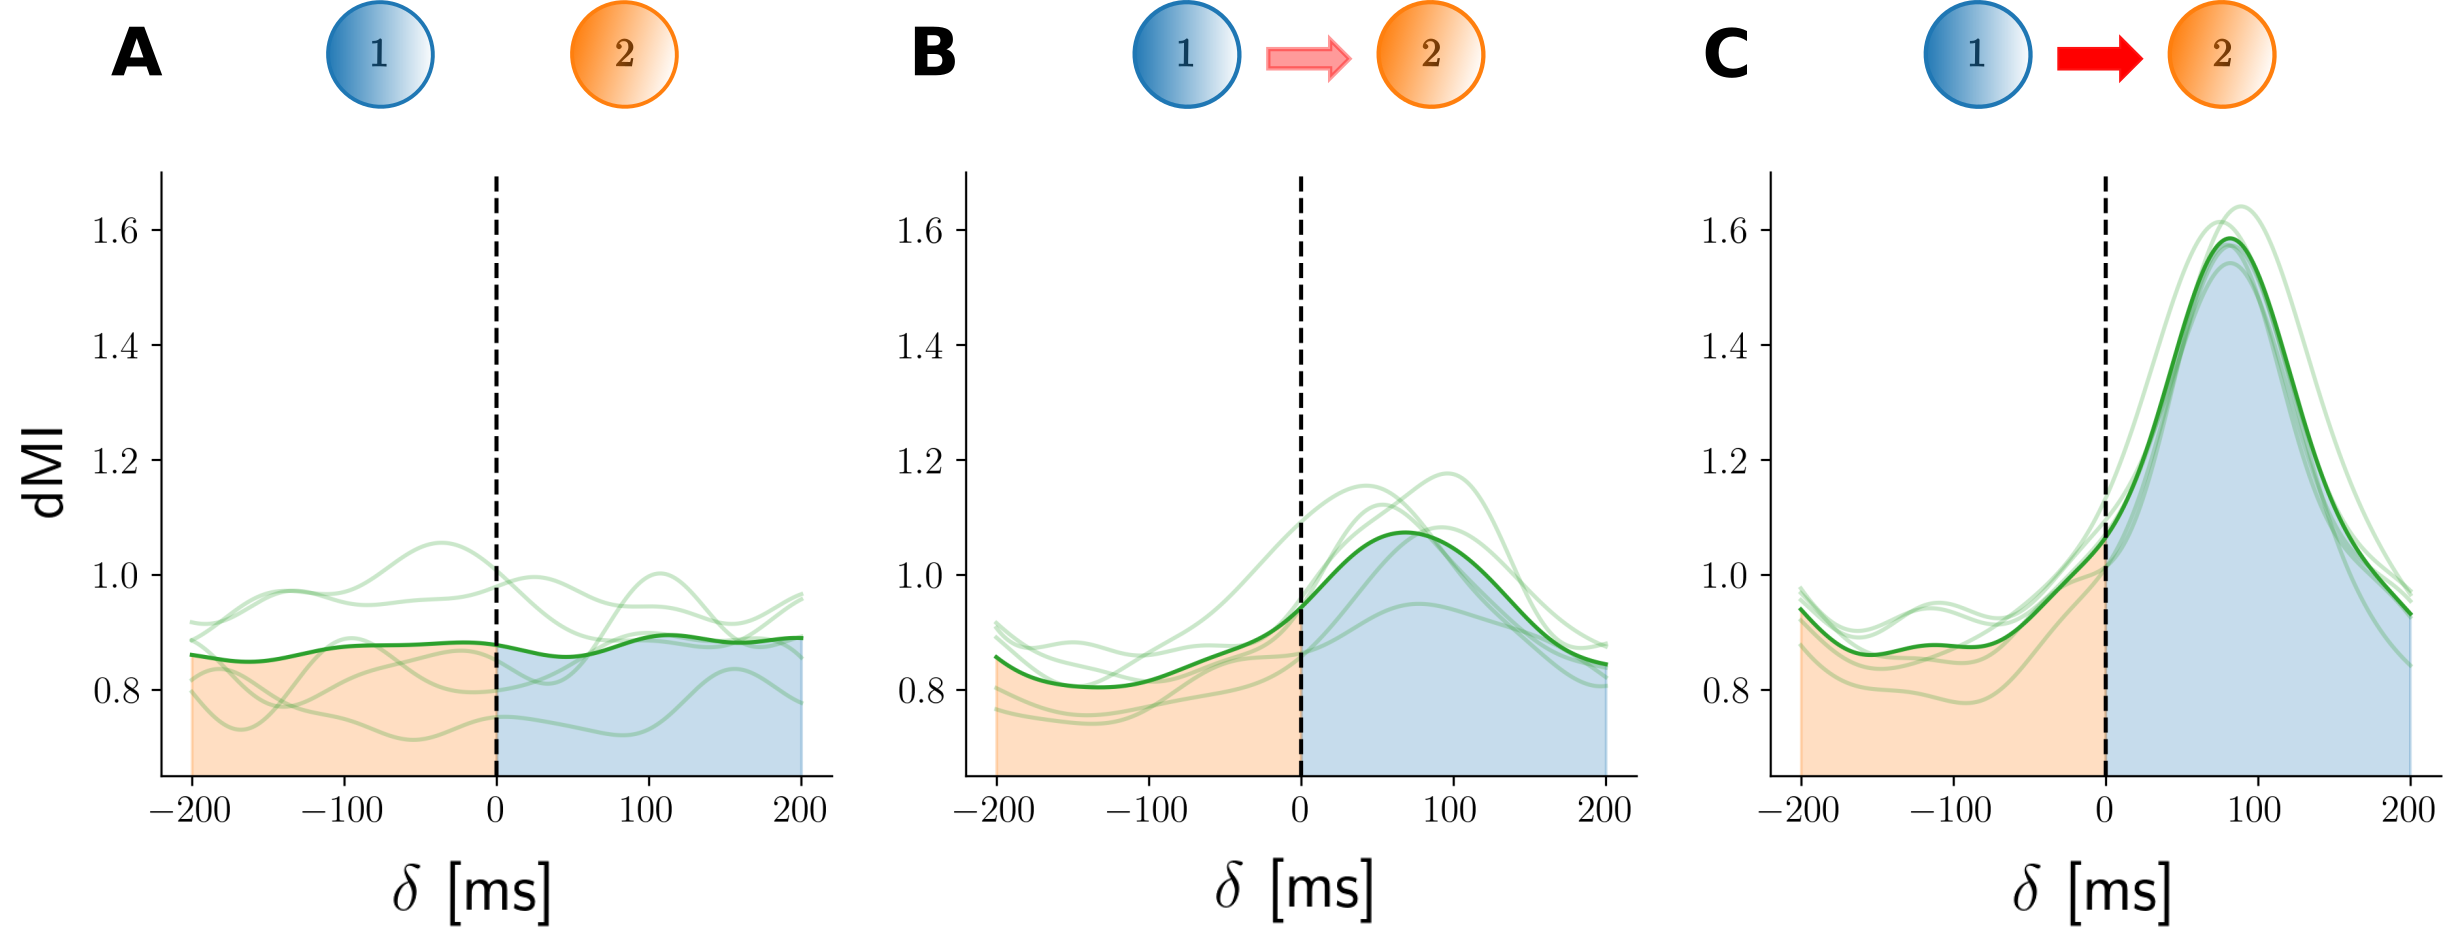
\includegraphics[width=\textwidth]{chapter2/figures/slow_stimulation.png}
    \caption{\textbf{Time-delayed mutual information}.
    Examples of dMI for different scenarios: ineffective transmission from 1 to 2 (A), clear transmission from 1 to 2 (B), and enhanced transmission from 1 to 2 (C).
    These examples were computed in the V-motif circuit by injecting slow modulation into population 1, with a delay of 6 ms, and $\Delta I$ values of -0.5, 0.0, and 0.5 $\mu$A/cm$^2$, respectively.
    The blue shaded area reflects the amount of information associated with the directionality 1 to 2, while the orange shaded area reflects the directionality 2 to 1.
    Solid green line indicates the average of the dMI over five different realizations.}
    \label{fig:slow-modulation-examples}
\end{figure}
Additionally, the value of this quantity indicates the strength of information transmission.
Figure \ref{fig:slow-modulation-examples} illustrates three examples of the transmission strength in the V-motif circuit under the influence of a slow modulation.
% The number of bins of the probability distributions were computed by the algorithm described in \citep{hacine2012low}.
%The theoretical description in \eqref{eq:difference_dMI} integration limits from or to infinity.
%With time series with a finite number of samples, this is not possible. 
Since the time series we analyzed are oscillatory with a well-defined frequency, 
we set the maximum time lag $\delta$ to be 200 ms, which corresponds to the period of the slow modulation (5 Hz).
Additionally, to determine the statistical significance we performed surrogate test analysis.
We generated 5000 surrogates using a time series permutation technique to obtain the null hypothesis distribution \citep{cohen2014analyzing}.
After that, $\Delta MI(x,y)$ values whose p-values were more than 0.05 were removed as indicative of no statistical significance.

\subsubsection{Fast signal injection}
When examining the transmission of a fast signal, we assessed the quality of the transmitted signal by utilizing the phase response curve (PRC) of the oscillating populations.
The PRC is defined as the phase shift of an oscillation caused by an external perturbation, relative to the unperturbed state, as a function of the time at which the perturbation is applied \citep{ko_phase-response_2009}.
It is commonly defined for isolated oscillators; however, in our system, each population represents a collective oscillator coupled to one or two other populations.
Consequently, measuring the response of a population to an injected pulse requires a different approach from that in the isolated case.
Recent studies have proposed techniques to measure information directionality based on PRCs in a circuit consisting of two mutually coupled oscillators under weak coupling conditions \citep{dumont_macroscopic_2019}.
The effect of an external perturbation on the sender population is quantified by the local phase response curve (lPRC), while the receiver populations are characterized by the non-local phase response curve (nPRC) 
\citep{schultheiss2011phase,pariz_transmission_2021}.
The nPRC represents the response of an oscillator to a non-local perturbation.
To determine the nPRC, a similar process to the PRC is followed.
Initially, the peaks of the firing rate for all populations are computed before applying the perturbation.
Then, a perturbation pulse is applied at different phases ($\beta$) to all excitatory neurons in the first population, altering the oscillation period, which subsequently affects the oscillation periods of other populations.
% These phase changes propagate to the other populations, affecting their oscillation periods.
% The axon delay time between populations is an important factor to consider.
% The response of the first population to the applied pulse takes an axon delay time ($\tau$) to reach the second population.
The delay $\tau$ between populations is crucial, as it takes that time for the response of the first population to reach the second population.
By subtracting the oscillation periods of the second and third populations, with and without the injected perturbation on the first population, we obtain the nPRC.
In our study, we went one step further.
Instead of applying the pulse at different phases and repeating the simulation to find the nPRC, we distributed the phase of the injected pulse along the oscillating period of the receiver population, treating the perturbation as a fast applied signal.
Each pulse had a width of 2 ms and an amplitude of 0.25 $\mu$A/cm$^2$.

We then quantified the information transmission $Z_i$ as
\begin{equation}
        Z_i = \displaystyle\int_{0}^{2\pi} |\text{nPRC}_i(\beta) | d\beta.
\end{equation}
% where the nPRC measurements were first fitted to a 4th-order Fourier series function for noise reduction.

\begin{figure}[!htb]
    \centering
    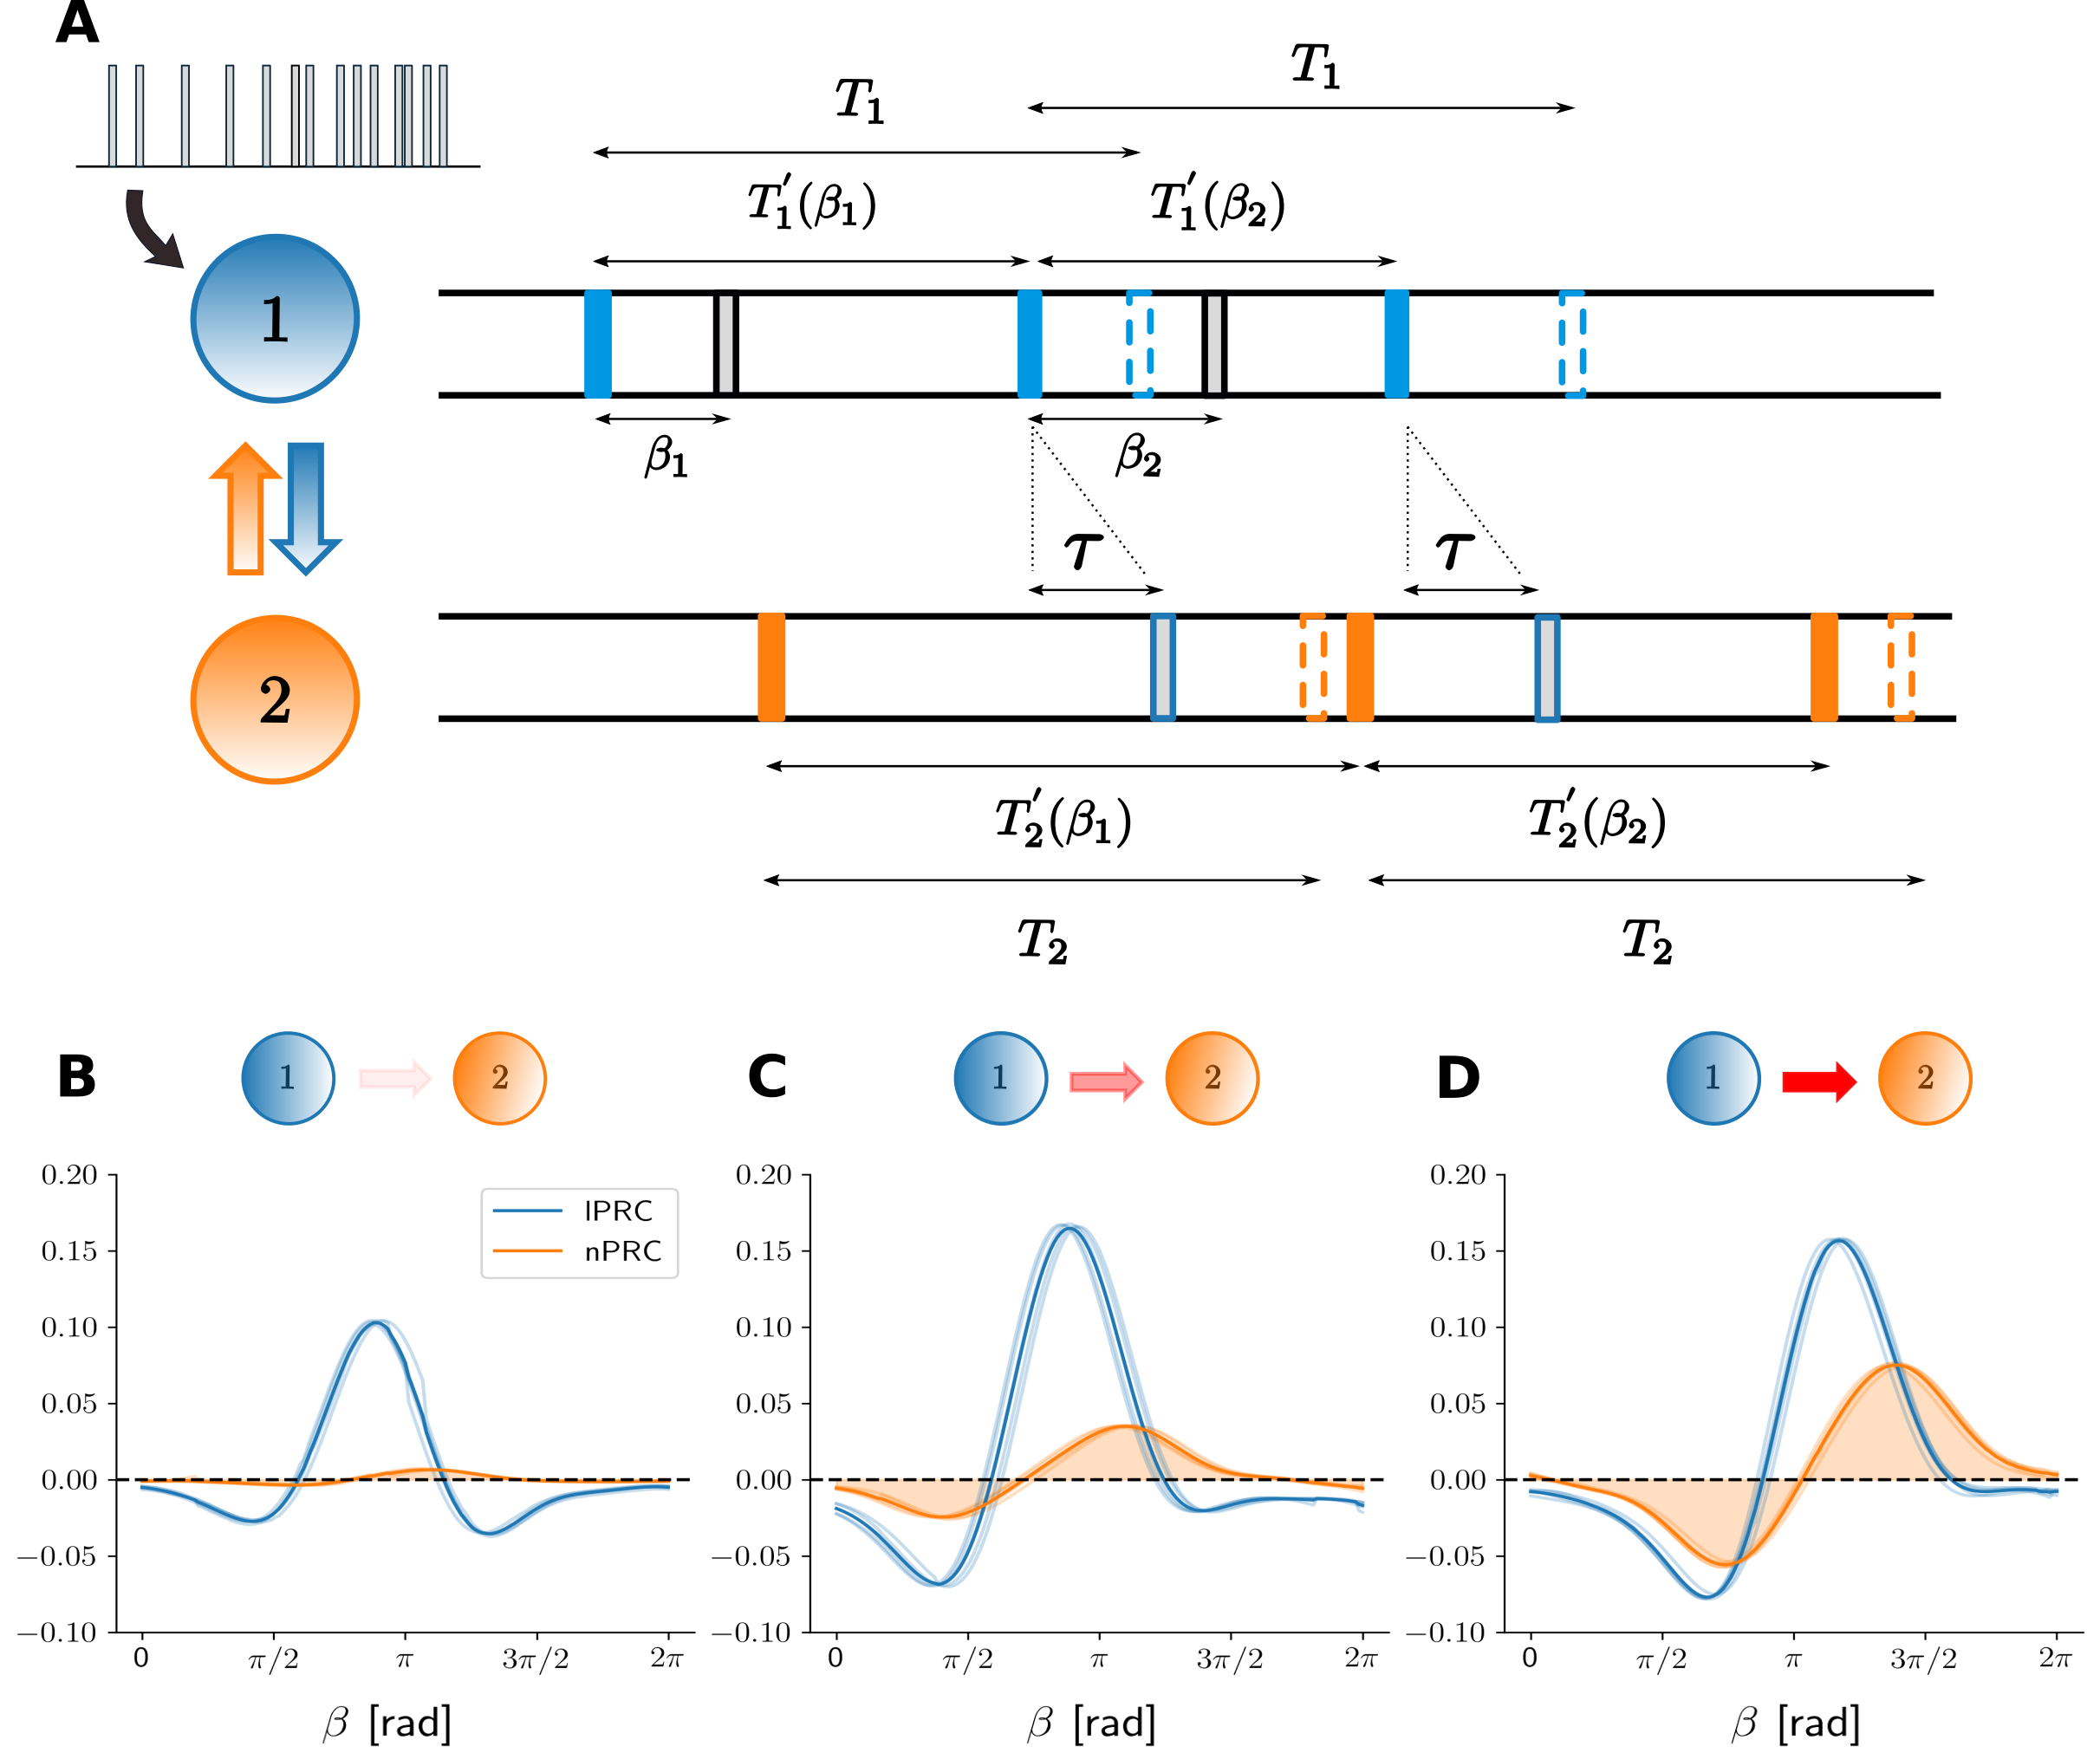
\includegraphics[width=\textwidth]{chapter2/figures/fast_stimulation.png}
    \caption{\textbf{lPRC and nPRC}.
    Schematics illustrating the computation of the phase response curves for the emitter population 1 (lPRC) and the receptor population 2 (nPRC).
    The injection of a pulsatile train into population 1 alters the regular spike generation, subsequently affecting the receptor population 2.
    The first pulse is injected with a phase $\beta_1$ while the second with a phase $\beta_2$.
    The perturbation arrived into population 2 after the time delay $\tau$ of the response of population 1.
    Three examples are provided, depicting the nPRC area, indicating no transmission (B), low transmission (C), and high transmission (D).
    These examples were computed in the V-motif circuit by
    injecting a pulsatile signal into population 1, with a delay of 6 ms, and $\Delta I$ values of
    -0.5, 0.0, and 0.5 $\mu$A/cm$^2$, respectively.
    Solid lines indicate the average over five different realizations.}
    \label{fig:fast-stimulation}
\end{figure}
Figure \ref{fig:fast-stimulation} illustrates the schematics representation of the computation of the lPRC and nPRC (A), and three different scenarios with different effective transmission (B, C and D).
\subsection{Simulations}
We implemented the numerical simulations using the Milstein algorithm \citep{milshtejn_approximate_1975} with a time step of $\Delta t$ = 0.01 ms.
The duration of the simulations varied depending on the speed of the applied modulation.
For slow signal modulation, we employed a simulation time of 6 seconds, while for fast signals, it was reduced to 4 seconds.
Throughout the simulations, we systematically explored the inter-population delay $\tau$ and the detuning or frequency mismatch $\Delta \nu$ (or $\Delta I$) of the sender population (space parameters).
All simulations were performed using the Python-based Brian simulator \citep{goodman2009brian}.
\end{document}